\section*{Методы оптимизации нулевого порядка}
Задача многомерной безусловной оптимизации формулируется следующим образом: найти минимум функции $f(x)$, где $x \in {R^n}$, при отсутствии ограничений на $x$, при этом $f(x)$ это скалярная целевая функция, непрерывно дифференцируемая ~\cite{b1}.

Все методы решения задач безусловной оптимизации состоят в том, что строится последовательность точек $\{x^n\}$ таким образом, чтобы последовательность функций $f(x^{(n)})$ была убывающей. На $k$-ом шаге ($k>0$) определяется вектор $\vec {S_k}$, в направлении которого функция $f(\overline{x})$ уменьшается. В этом направлении делается шаг величиной $\lambda_k$ и находится новая точка:
\begin{equation}
	x^{(k+1)} = x^k + \vec{S_k} \lambda_k, \hspace{50pt} f(x^{k+1}) < f(x^k).
\end{equation}
Последовательность $\{x^{(n)}\}_{n \in N}$, удовлетворяющая условию, называется релаксационной последовательностью, а соответствующие методы -- методами спуска. Методы решения делятся на методы с использованием информации о производных функции и без. Различные методы спуска отличаются выбором направления и величины шага ~\cite{b1}.

К методам нулевого порядка относятся методы, не использующие производные для выбора направления спуска: метод Гаусса, метод вращающихся направлений (Розенброка); метод деформируемого многогранника (поиска по симплексу); метод Хука Дживса, метод Пауэлла ~\cite{b1}.

Метод Гаусса-Зейделя (покоординатный спуск): обеспечивает сходимость к локальному минимуму для гладких функций. Недостаток: может делать мелкие шаги при минимизации «овражных» функций (рис. ~\ref{img:1-1}).

Метод Хука-Дживса: легко реализуется и эффективен для сложных функций. Недостаток: медленная сходимость при «овражных» функциях (рис. ~\ref{img:1-1}) и зависимость от выбора ускоряющего множителя.

Метод вращающихся направлений (Розенброка): эффективно определяет движение вдоль дна оврага (рис. ~\ref{img:1-1}). Недостаток: может требовать больших вычислительных затрат для построения нового базиса.

Метод поиска по симплексу (Нелдера-Мида): простота и малое количество параметров. Недостаток: может приводить к бесконечным последовательностям поисков.

Методы сопряжённых направлений (Пауэлла): быстрая сходимость для квадратичных функций. Недостаток: требуют решения громоздкой задачи на собственные значения матрицы.

\begin{figure}[H]
	\centering
	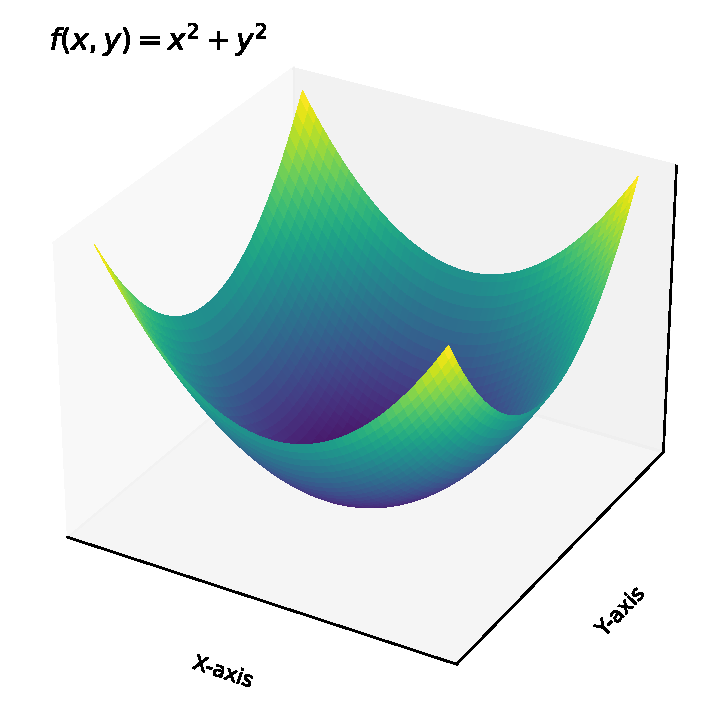
\includegraphics[width=0.3\textwidth, trim=0 0 0 0]{img/1-1.pdf}
	\caption{Пример овражной функции}
	\label{img:1-1}
\end{figure}

\section*{Список использованных источников}
\printbibliography[heading=none]